\cleardoublepage
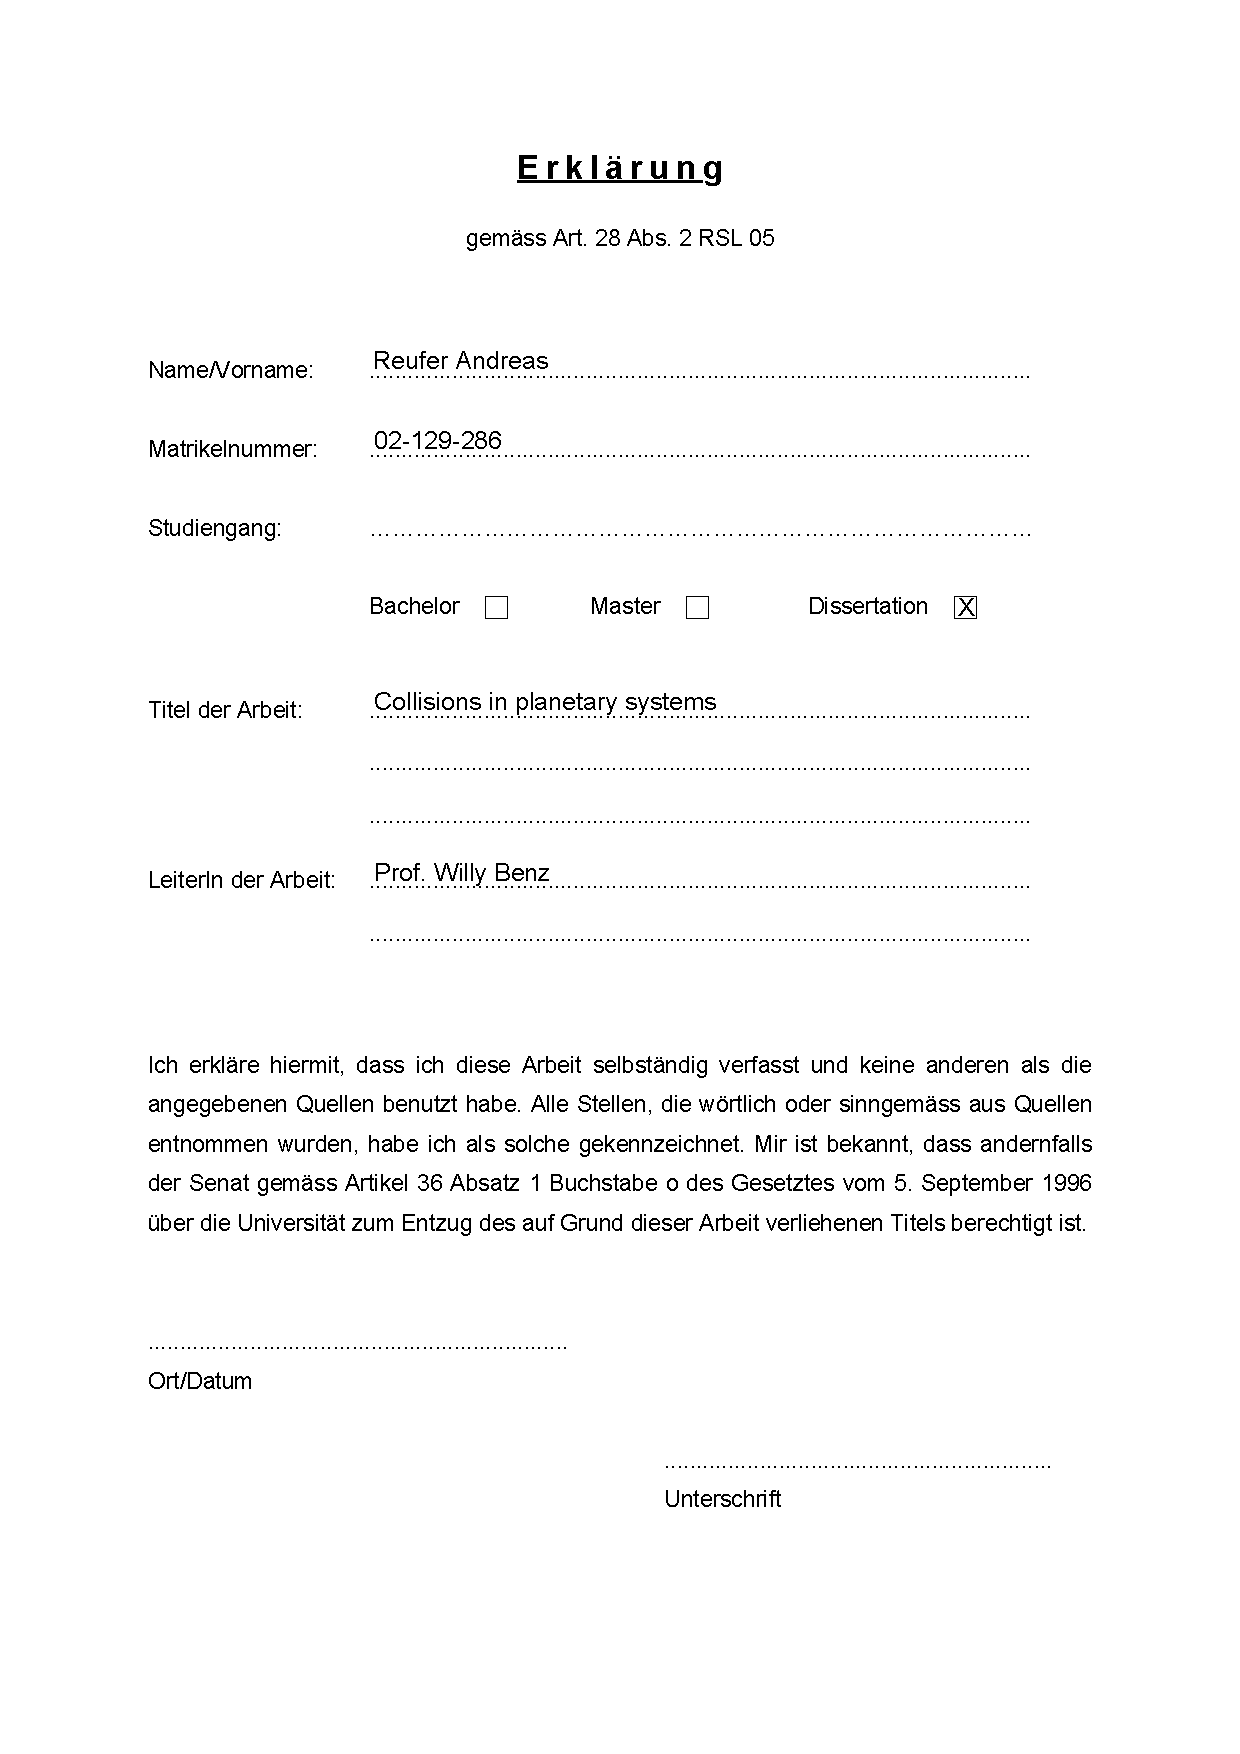
\includepdf[fitpaper=true]{00figs/PhD_declaration_ger.pdf}

%\cleardoublepage
\chapter*{Curriculum vitae}

\begin{tabular}{r p{12.0cm}}
\multicolumn{2}{l}{ {\large \bf Personal data} } \\
Full name & Andreas Reufer\\
Date of birth & 19.02.1982\\
martial status & not married \\
Address & Standstrasse 25, \\
 & 3014 Bern, Switzerland \\
\\
\multicolumn{2}{l}{ {\large \bf Education} } \\
1989 - 1995 & Primary and secondary schools in Köniz and Liebefeld\\
1995 - 2001 & Gymnasium Köniz, Major in Mathematics and Physics\\
\\
\multicolumn{2}{l}{ {\large \bf Academic record} } \\
2002 - 2007 & Studies in physics, mathematics and theory of science, University of Bern \\
2006 - 2007 & Diploma thesis in physics: \emph{Dynamics of planets in gaseous disks}, marked \emph{summa cum laude} \\
2007 - 2011 & PhD thesis in physics: \emph{Collisions in planetary systems} \\
%\\
%\multicolumn{2}{l}{ {\large \bf Languages} } \\
%German & mother tongue\\
%English & fluent, spoken and written\\
%French & basic knowledge, spoken and written \\
\end{tabular}

